\begin{frame}{R-squared ($R^2$ or $r^2$) —\\ Coefficient of Determination}
    \small
    \begin{itemize}
        \item \textbf{A statistical metric} used to measure how well the independent variables explain the variability in the dependent variable.
        \item It provides a measure of the goodness-of-fit (\textbf{performance}) for a regression model:
    \end{itemize}

    \begin{equation*}
        R^2 = 1 - \frac{\text{SS}_{\text{res}}}{\text{SS}_{\text{tot}}}
    \end{equation*}

    \textbf{Where:}
    \begin{itemize}
        \item $\text{SS}_{\text{residual}} = \sum (y_i - \hat{y}_i)^2$: sum of squared residuals (difference between observed and predicted values).
        \item $\text{SS}_{\text{total}} = \sum (y_i - \bar{y})^2$: total variation in the data around the mean.
    \end{itemize}
\end{frame}



\begin{frame}{Visualisation of $R^2$}
    \begin{columns}
        \column{0.55\textwidth}
            \begin{figure}
                \centering
                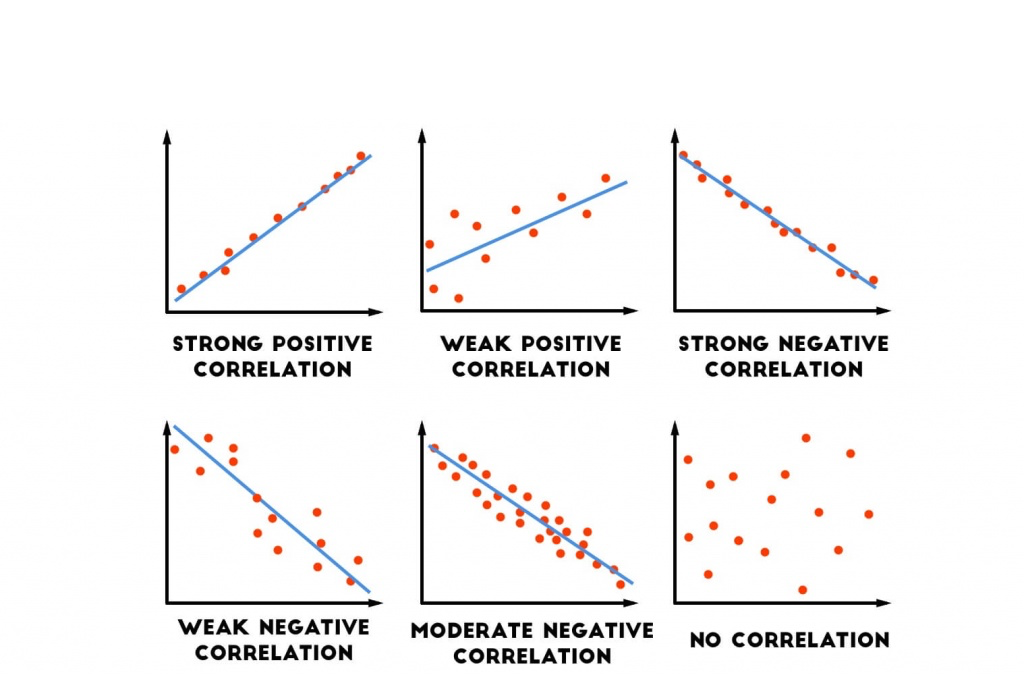
\includegraphics[width=\linewidth]{images/linear-regression/linear-regression-20.png}
            \end{figure}
        
        \column{0.45\textwidth}
            \textbf{Interpretation:}
            \begin{itemize}
                \item $R^2 = 1$: The model perfectly explains the data.
                \item $R^2 = 0$: The model explains none of the variability (as good as guessing the mean).
                \item $R^2 < 0$: The model performs worse than a simple horizontal line at the mean of the target variable.
            \end{itemize}
    \end{columns}
\end{frame}


\begin{frame}[allowframebreaks]{Properties of $R^2$}

\textbf{Range:}
\begin{itemize}
    \item $0 \leq R^2 \leq 1$
    \begin{itemize}
        \item $R^2 = 1$: Perfect model; predictions perfectly match the observations.
        \item $R^2 = 0$: Model does no better than the mean of the dependent variable.
    \end{itemize}
\end{itemize}

\textbf{Interpretability:}
\begin{itemize}
    \item $R^2$ indicates the proportion of the variance in the dependent variable that is predictable from the independent variables.
\end{itemize}

\textbf{Limitations:}
\begin{itemize}
    \item $R^2$ increases with the addition of independent variables, even if they don’t improve model prediction significantly.
    \item Does not account for overfitting or the complexity of the model.
\end{itemize}

\textbf{Negative Values:}
\begin{itemize}
    \item In rare cases, $R^2$ can be negative when the model fits the data worse than a horizontal line representing the mean of the dependent variable.
\end{itemize}

\textbf{Adjusted $R^2$:}
\begin{itemize}
    \item Adjusted $R^2$ penalizes for the addition of non-significant predictors and is often a better metric for comparing models.
    \item Here, $n$ is the number of data points and $p$ is the number of predictors:
\end{itemize}

\begin{equation*}
    R^2_{\text{adj}} = 1 - \frac{(1 - R^2)(n - 1)}{n - p - 1}
\end{equation*}

\end{frame}


\begin{frame}{R-squared vs. Cost Function}

\textbf{R-squared vs. Cost Function:}
\begin{itemize}
    \item \textbf{Cost Function:} A mathematical function used to optimize a model during training by minimizing the prediction error (e.g., Mean Squared Error or MSE).
    \begin{itemize}
        \item Example: Gradient Descent minimizes MSE for linear regression.
    \end{itemize}
    \item \textbf{R-squared:} A metric to evaluate how well the model fits the data \textbf{after training}. It is not used during model optimization.
\end{itemize}

\textbf{Limitations of $R^2$:}
\begin{enumerate}
    \item \textbf{Doesn't Indicate Causation:} A high $R^2$ doesn’t mean the predictors cause the dependent variable.
    \item \textbf{Sensitive to Overfitting:} A complex model might have a high $R^2$ but poor generalization.
    \item \textbf{Adjusted $R^2$:} For models with many predictors, use adjusted $R^2$, which accounts for the number of predictors to avoid overestimating performance.
\end{enumerate}

\end{frame}
